%*************************************************************************
% Dokument Einstellungen
%*************************************************************************
\documentclass[fontsize=12pt,paper=a4,open=any,parskip=half,
  twoside=false,toc=listof,toc=bibliography,fleqn,leqno,
  captions=nooneline,captions=tableabove,british]{scrbook}
%*************************************************************************
% Importieren von Paketen die benutzt werden
%*************************************************************************
\usepackage[utf8]{inputenc} % load early
\usepackage[T1]{fontenc}    % load early
\usepackage[ngerman]{babel}
\usepackage[autostyle=true]{csquotes}
\usepackage{graphicx, booktabs, float, scrhack}
\usepackage{caption}
\usepackage{listings}
%\usepackage{fancyref}
%\usepackage{showkeys}
\usepackage[svgnames]{xcolor}
\usepackage{amsmath,amssymb}
\usepackage[automark]{scrlayer-scrpage}
\usepackage[backend=biber,style=alphabetic]{biblatex} %,sortcase=false,

%*************************************************************************
% Bibliographies - Zitatquellen
%*************************************************************************
\addbibresource{Projekt.bib}

%*************************************************************************
% Weitere Dokument Einstellungen
%*************************************************************************
\PassOptionsToPackage{hyphens}{url} 
\usepackage[hidelinks]{hyperref}  % load late
\setkomafont{disposition}{\sffamily}
\setcounter{secnumdepth}{3}
\addtocontents{toc}{\setcounter{tocdepth}{1}}
%*************************************************************************
% Dokumentanfang
%*************************************************************************
\begin{document}
%Aktivierung römische Seitenzahlen
\frontmatter

%Titelblatt Einstellungen
\titlehead{% siehe KOMA-Script-Anleitung
  \begin{minipage}[t]{0.65\textwidth}
    \raggedright
    			Frankfurt University of Applied Sciences\\
				Fachbereich 2: Informatik und Ingenieurwissenschaften\\
				Studiengang: Informatik (B.Sc.)\\
  \end{minipage}
  \hfill
  \raisebox{-\dimexpr\totalheight-\ht\strutbox\relax}{
    
\includegraphics[width=5cm]{Bilder/fra-uas}
  }
}

\subject{Projektarbeit}
\title{Software-defined Networking mit Openflow}
\subtitle{}
\author{Mücahit Sagiroglu\\
Matrikelnummer: 1228852\\
James Belmonte\\
Matrikelnummer: 1340604\\
Naghmeh Ghavidel Rostami\\
Matrikelnummer: 1249307\\
Tung Trinh\\
Matrikelnummer:\\
}
\date{Vorgelegt am: 27. Januar 2022}
\publishers{Dozent: Maurizio Petrozziello\\
Modul 25: Informatik Projekt\\
Software-defined Networking mit Openflow\\
Wintersemester 2021/2022\\
}

\maketitle
%Eigenständigkeitserklärung
\chapter*{Eigenständigkeitserklärung}
Hiermit erklären wir, dass wir die vorliegende Arbeit eigenständig verfasst, keine anderen als die
angegebenen Quellen und Hilfsmittel verwendet sowie die aus fremden Quellen direkt oder indirekt
übernommenen Stellen/Gedanken als solche kenntlich gemacht haben. Diese Arbeit wurde noch keiner
anderen Prüfungskommission in dieser oder einer ähnlichen Form vorgelegt. Sie wurde bisher auch nicht
veröffentlicht.

Hiermit stimmen wir zu, dass die vorliegende Arbeit von der Prüferin/ dem Prüfer in elektronischer Form
mit entsprechender Software auf Plagiate überprüft wird.

\begin{figure}[H]
	\centering
	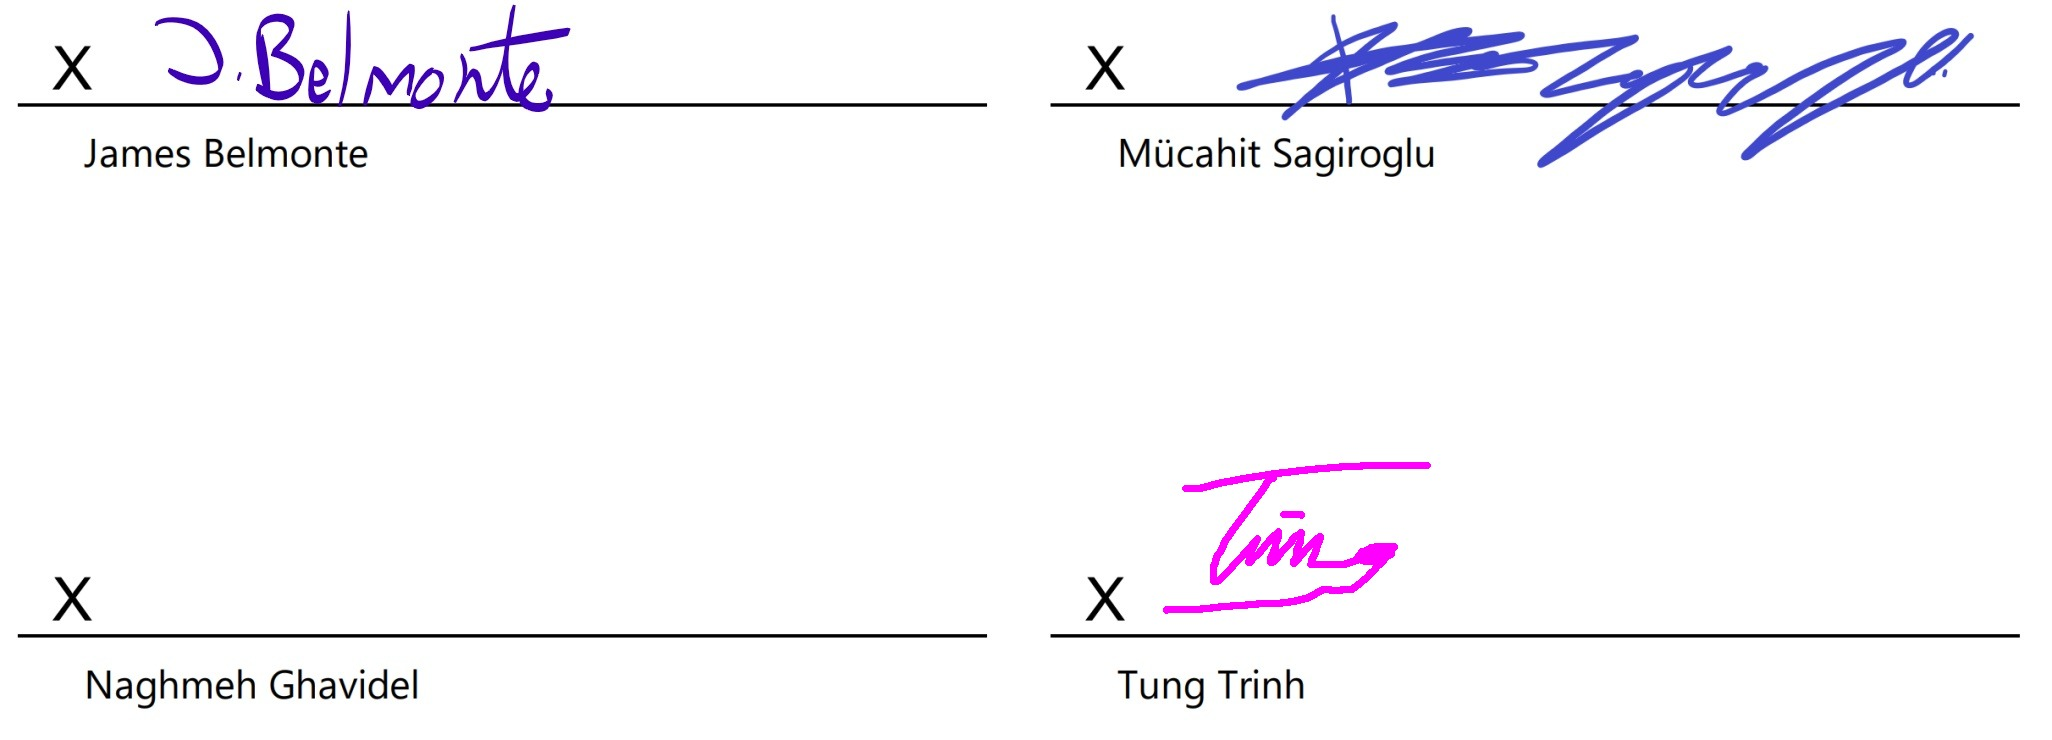
\includegraphics[width=1\linewidth]{Bilder/unterschrift}
\end{figure}

%Inhaltsverzeichnes & Abbildungsverzeichnis & Tabellenverzeichnis
\tableofcontents
\listoffigures
\listoftables
\lstlistoflistings

%Aktivierung arabische Seitenzahlen
\mainmatter % Seite fängt mit 1 an



%Kapitel: Einleitung
\chapter{Einleitung}\label{ch:intro}
Seit der Einführung des ... existiert das ..., welcher, wie der Name ausdrückt, einige ... für .... zur Verfügung stellt.

\section{Software-defined Networking}\label{sdn}
asd
\subsection{Einleitung von James}\label{einl-james}
asddsa
\subsection{Einleitung von Naghmeh}\label{einl-naghmeh}
asddsa
\subsection{Einleitung von Tung}\label{einl-tung}
asddsa
\subsection{Einleitung von Mücahit}\label{einl-müco}
asddsa

\section{Motivation}
Was hat uns zum schreiben der Projektarbeit (in Bezug auf die Problemstellung) gebracht?

https://www.scribbr.de/aufbau-und-gliederung/motivation-bachelorarbeit/
\section{Problemstellung}
Die Problemstellung beschreibt das Forschungsproblem, das du mit deiner Abschlussarbeit lösen möchtest.
Was ist das Thema des Projekts und wie lautet die konkrete Fragestellung?

https://www.scribbr.de/anfang-abschlussarbeit/problemstellung/

Würde hier die Aufgabenstellungen hinschreiben, sollten irgendwo ja erwähnt sein.

\section{Aufbau der Arbeit}
Wie ist die restliche Projektarbeit aufgebaut? Was kommt noch?


\chapter{Projekt}
asd
\section{Projektziel}
Wie lautet das Ziel des Projekts?


Die Zielsetzung deiner Bachelorarbeit sollte deinen Lesenden einen Einblick in das „Warum“ und das „Wie“ deiner Untersuchung geben.

Warum führst du die Forschung durch und wie wirst du dieses Ziel erreichen?

https://www.scribbr.de/anfang-abschlussarbeit/zielsetzung-formulieren/

\section{Vorgehen}
Wie sieht die Vorgehensweise aus?
\section{Festlegen von Meilensteinen}
Welche Meilensteine wurden festgelegt?

\section{Verwendete Werkzeuge}
Text
\subsection{Mininet}
vllt. Text
\subsubsection{Einführung}
Mininet ist ein Netzwerk Emulator mit der man Netzwerke simulieren kann. Bei Mininet handelt es sich um kostenlose Open-Source-Software, die die virtuelle Maschine und Controller die Recherche in SDN und OpenFlow ermöglichen.
Mininets ermöglichen eine sehr groß angelegte Topologie, wodurch ein Netzwerk von Hosts, Switch-, Controller- und virtuelle Links erstellt wird. Das Ausführen von Tests mit den Komponenten ist unkompliziert und kann über Python Schnittstelle erledigt werden.
\subsubsection{Funktionalität}
•      Mininet stellt ein einfaches Netzwerk Testbed dar, welches aber auch gleichzeitig auch günstig ist. Da der Switch Openflow in Mininet alle Eigenschaften hat, wie ein echter switch OpenFlow, ist die Anwendung von Netzwerkemulator mit Mininet praktisch sinnvoll.
•      Ermöglicht das Debuggen und Ausführen von Tests großer Netzwerke mithilfe von CLI.
•      Unterstützung zum Einrichten beliebiger benutzerdefinierter Diagramme
•      Die Anwendungen im Mininet können im echten Netzwerk realisiert werden, ohne dass man sein Code ändern muss.
•      Mininet bieten eine benutzerfreundliche und erweiterbare Python-API

\subsubsection{Nachteil}
Aktuelle Nachteile von Mininet: nur unter Linux lauffähig. Dadurch, dass Mininet nur auf einem Rechner ausgeführt werden kann, ist es leistungsmäßig eingeschränkt. Daher hängt die Leistung von den Ressourcen dieses Rechners ab.
\subsubsection{Komponenten}
•      Links: Die Links in einem Mininet sind ein Paar virtueller Ethernets, die wie ein Draht funktionieren, der zwei virtuelle Schnittstellen verbindet. Pakete werden von einer Schnittstelle zur anderen gesendet, diese Schnittstellen stellen für alle genau dasselbe wie Ethernet-Ports dar System- und Anwendungssoftware.
•      Hosts: Die Netzwerk-Namespaces enthalten den Netzwerkstatus (network state). Sie bieten Prozessen (oder Gruppen von Prozessen) die Kontrolle über Schnittstellen, Ports und Routing-Tabellen. Jeder Host hat seine eigenen Ethernet-Schnittstellen (initiiert und gesetzt durch den Befehl ip link add/set) und eine Verbindung zum Mininet.
•      Switches: OpenFlow-Softswitches bieten die gleiche Semantik für das Senden
Paket wie ein Hardware-Switch. Ein Switch arbeitet auf der Datenverbindungsschicht (Layer 2) und manchmal auf der Netzwerkschicht (Layer 3) des OSI (Open Systems Interconnection) -Referenzmodells und unterstützt daher jedes beliebige Paketprotokoll. LANs, die zur Verbindung von Segmenten Switches verwenden, werden als geswitchte LANs oder, im Falle von Ethernet-Netzwerken, als geswitchte Ethernet-LANs bezeichnet. In Netzwerken ist der Switch das Gerät, das Pakete zwischen LAN-Segmenten filtert und weiterleitet
•      Controller: Controller können sich überall im realen Netzwerk oder in der Umgebung befinden Simulation.
\subsubsection{Installation}
sudo apt-get install git
git clone git://github.com/mininet/mininet
sudo mininet/util/install.sh –a
\subsubsection{Aufbau}
Durch die Eingabe von dem Befehl sudo mn erfolgt ein Default Mininet. Auf der virtuellen Maschine laufen 4 Entitäten (2 Hosts, 1 Switch, 1 Controller).

\subsection{Floodlight}
vllt. Text
\subsubsection{Einführung}
Derzeit gibt es auf dem Markt einige Controller, die in SDN verwendet werden, wie zum Beispiel: OpenDaylight,Ryu, POX, NOX, HP VENTIL...            Wir haben uns für Floodlight Controller entschieden, weil er die Anforderungen des Projekts erfüllt und einfach zu installiert ist. Floodlight Controller ist sehr user-friendly und bietet sogar eine Benutzeroberfläche.
\subsubsection{Funktionalität}
Text
\subsubsection{Nachteil}
Text
\subsubsection{Komponenten}
Modules etc.
\subsubsection{Installation}
git clone git://github.com/floodlight/floodlight.git
cd floodlight
git submodule init
git submodule update
ant
\subsubsection{Aufbau}
java -jar target/floodlight.jar

\subsection{Ergebnis}
Text. Please insert a picture of floodlight GUI
Zeigen was am Ende mit Controller und Mininet erreicht wird.



\chapter{Durchführung des Projektes}
Erklären Controller-Auswahl!
Projektdurchführung
Würde in diesem Bereich die Lösungen hinschreiben, jeweils für jede Aufgabe eine section. Beispielsweise wäre die erste section Netzwerkplan



\section{Netzwerkplan}
\subsection{Vorüberlegung}
Das Netzwerkmodell umfasst:
Mininet: 4 Switches und 40 Hosts erstellen. Diese Switches und Hosts werden verbunden mit unserem Floodlight Controller. 4 Switches repräsentieren 4 Lokationen mit jeweils 10 Hosts. Damit die Hosts und Switches mit dem Internet verbunden werden können, steht 4 Routers da. Router kann man wie ein Gateway betrachten. Anhand von Headern und Weiterleitungstabellen bestimmt der Router den besten Weg zur Weiterleitung der Pakete.
Floodlight Controller: SDN-Controller (SDN-Controller) steuert den Zugriff zwischen Hosts im Netzwerk. Dies wird durch eine Python Datei implementiert

\begin{figure}[htbp]
 \centering
 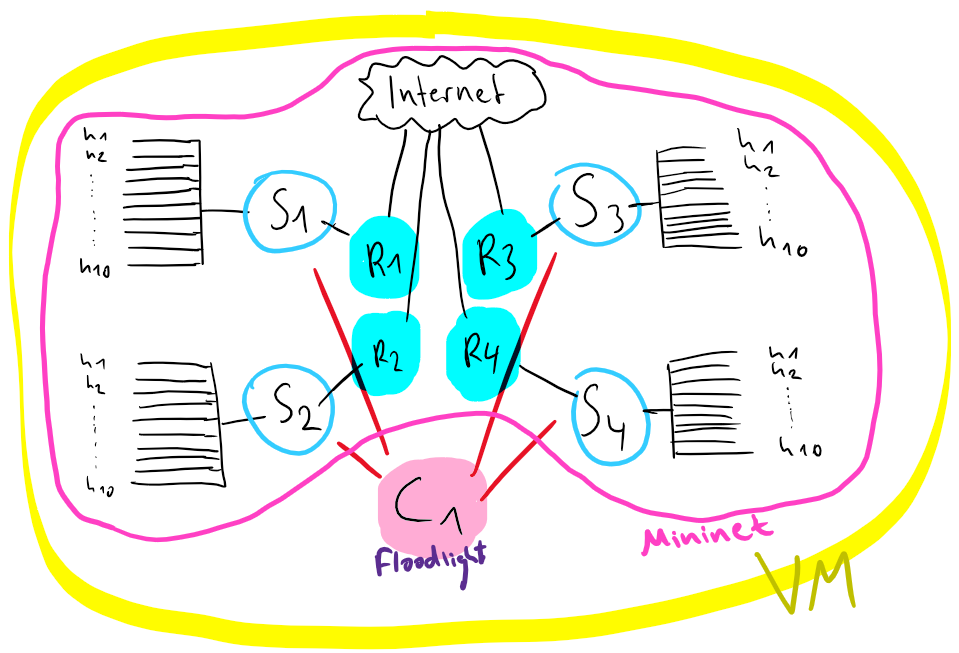
\includegraphics[width=1.0\textwidth]{Bilder/prototyp}
 \captionsetup{justification=centering,margin=2cm}
 \caption{Netzwerkplan unseres Unternehmens}
 \label{networkplan}
\end{figure}

\subsection{Durchführung}


\begin{figure}[htbp]
 \centering
 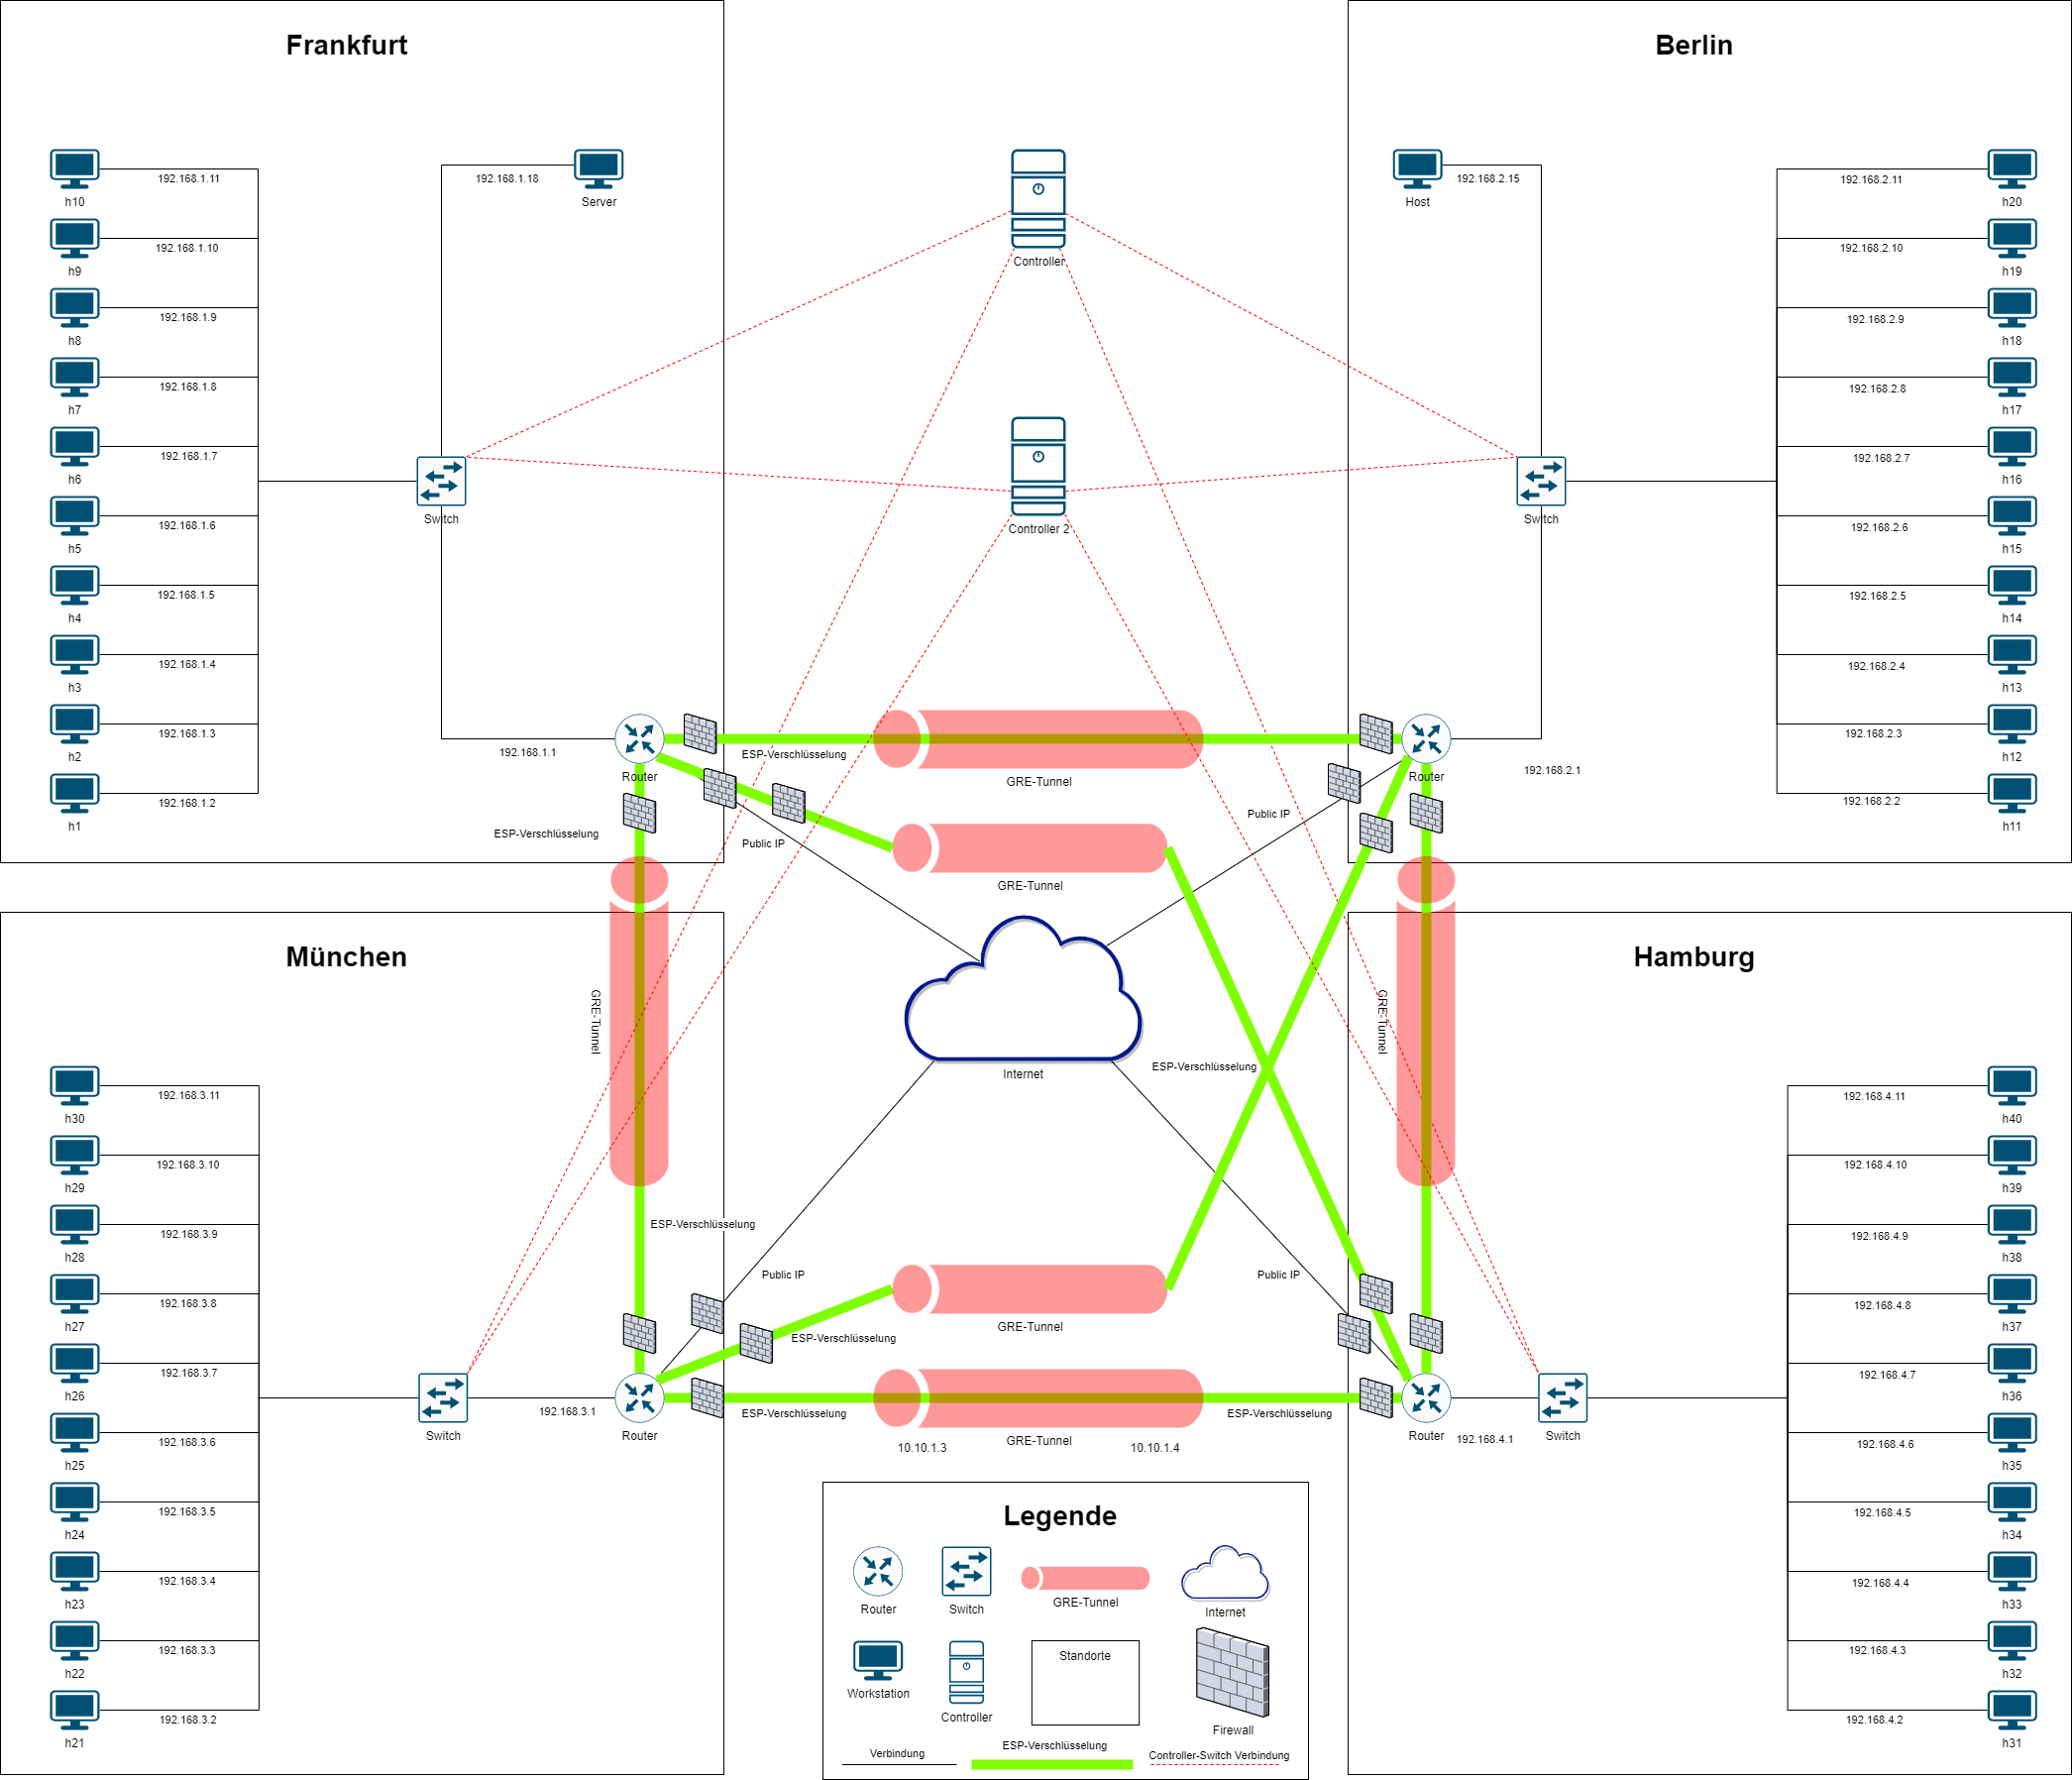
\includegraphics[width=1.0\textwidth]{Bilder/netzwerkplan}
 \captionsetup{justification=centering,margin=2cm}
 \caption{Netzwerkplan unseres Unternehmens}
 \label{networkplan}
\end{figure}

\section{Aufbau des Netzwerkgerüstes in Mininet}
\subsection{Durchführung}
In diesem Abschnitt wird der Aufbau der Simulation über Mininet erklärt.
 
In der Main-Funktion werden die Komponenten eines Netzwerks deklariert und aufgerufen. Das sind eine Topologie, ein Controller mit zugewiesenem Port und ein Mininet Objekt mit der deklarierten Topologie. Anschließend geben wir für unsere Routers Routing-Regeln und Informationen.

\subsection{Aufbau der Topologie}
Der Mininet-Script besteht aus einer Main-Funktion bei der als allererstes mit der von uns definierten Klasse „Netzwerk()“. Und damit zeigen wir wie das Netzwerk beziehungsweise eine Topologie erstellt wird. Die Klasse übernimmt ein Topo-Objekt an dem er mit der in ihm definierten „build()“ Methode die Konfiguration des Netzwerkes vornimmt. 
 
In der „build()“ Methode definieren wir zuerst einen String der den privaten-IP-Bereich der vier Lokationen enthält. Der defaultIP String bleibt in unvollständiger Form „192.168.\%s.1/24“. Somit kann er später durch passende Stellen ersetzt und genutzt werden. Lediglich ist hier im dritten Block ein Platzhalter eingesetzt der beim erstellen der Router in einer Schleife durch die Zahl der Iteration ersetzt wird.
 
Zunächst wird ein leeres Array/Liste unter dem Namen „Routers“ deklariert. Dies wird dann später genutzt und mit den Router-Objekten gefüllt. Später für die Verlinkung der Router mit dem jeweiligen Switch wird die Liste aufgerufen. Für große Anzahl von Router ist die Bedeutung der Liste sehr praktisch.
 
Im nächsten Teil der Klasse Netzwerk, Zeile 35 bis 53 wollen wir die Komponenten des Netzwerks implementieren. Dies ist mit Hilfe einer Schleife mit 4 Durchläufe ausgeführt worden. 4 Durchläufe entsprechen 4 Lokationen, jeweils 1 Switch 1 Router und 10 Hosts.
Dabei wird bei jeder Iteration erst ein Router-Objekt mit der Methode „self.addNode()“ erstellt, bei dem der Name, der private IP-Adressen-Bereich, die MAC-Adresse und benutzerdefinierte Parameter für die Konfiguration, dass der Router IP-Forwarding aktiviert bekommt, übergeben. Danach wird der Router der vorher erstellten Liste eingefügt.
 
Als nächstes wird ein Switch mit der Methode „self.addSwitch()“ erstellt, der nur einen Namen erhält, der anschließend mit der Methode „self.addLink()“ mit dem Router verbunden wird, bei dem die Netzwerkschnittstelle des Router benannt und der private-IP-Adressenbereich vergeben wird.
 
Danach folgt noch eine Schleife, bei der insgesamt n Hosts erstellt und mit dem Switch verbunden werden. Die Hosts erhalten für den jeweiligen privaten-IP-Bereich eine IP, eine MAC-Adresse und die IP des jeweiligen Routers als Standard-Route zugewiesen. 
Nachdem für alle Lokationen der Rumpf erstellt worden ist, stellen wir die Verbindungen zwischen den Routern mit dem Befehl „self.addLink()“ her. Dabei wird jeder Router mit allen anderen Routern verbunden. Dieser Vorgang wird das Internet simulieren, worauf ebenfalls der Tunnel und die Verschlüsselung implementiert wird. Dabei wird der Netzwerkschnittstellen-Name für beide Router und die jeweilige öffentliche-IP-Adresse definiert. Zusätzlich setzen wir per „bw=20“ Befehl die Bandbreite der Leitung auf 20 Megabit, wobei dies die geforderte SDSL-Leitung der Aufgabe sieben darstellen soll. 

\subsection{Controller Implementierung}
Es würde weiter bei der Main-Funktion gehen. Dort initialisieren wir ein RemoteController-Objekt der einen Namen, die Konfiguration um was für einen Controller es sich handelt, die IP-Adresse und den Port, wo er zu erreichen ist, bekommt. Hier ist wichtig zu erwähnen, dass der Controller auf Ubuntu läuft und das der Controller per „localhost“ zu erreichen ist. Hier könnte man ebenfalls den Controller auf einer anderen VM laufen lassen und ihn per Internes Netzwerk verbinden oder auf der echten Welt laufen lassen und ihn per NAT-Verbindung verbinden. Auch besteht noch die Möglichkeit den Controller auf dem Betriebssystem, auf dem Virtualbox läuft, laufen zu lassen und ihn per Host-Only-Adapter zu verbinden. Anschließend wird ein Mininet-Objekt erstellt, bei dem die erstellte Topologie, der erstellte Controller, ein TCLink-Objekt für die Einstellung der Bandbreite der Netzwerkadapter und ein OVSKernelSwitch-Objekt für die Erstellung der Switche als Open vSwitche. Die Open vSwitche nutzen wir später, um den Quality of Service zu implementieren, bei dem wir per ovs-vsctl-Befehle Queues an den Ports der Switche erstellen und die Priorisierung der Pakete vornehmen. 

\subsection{Ergebnis}
Was haben wir dadurch erreicht. Zusammenfassen.
Was ist schief gelaufen?

\section{Verschlüsselung der Netzwerkverbindung zwischen den Lokationen}
Als nächstes folgt in der Main-Funktion die Einrichtung der Tunnel zwischen den Routern beziehungsweise den Lokationen. Dafür baut jeder Router mit jedem Router einen GRE-Tunnel auf, für den wir den Befehl „ip tunnel add Tunnel-Name mode gre local Router-Schnittstelle-des-eigenen-Routers remote Router-Schnittstelle-des-anderen-Routers ttl 255“ bei jedem Router mit der Mininet-Methode „info(net[‚Router-Name‘].cmd(Befehl))“ ausgeben und ausführen. Nachdem die Verbindung definiert wurde fahren wir den Tunnel-Adapter per „ip link set Tunnel-Name up“ hoch. Anschließend geben wir dem Tunnel Adapter mit dem Befehl „ip addr add Tunnel-IP dev Tunnel-Name“ die jeweilige Tunnel IP. Hier ist wichtig zu erwähnen, dass die IP zwischen zwei Lokationen im selben Netzwerkbereich, wie bei der Erstellung und Simulierung des Internets zwischen den Routern, sein muss. Nachdem der Tunnel aufgesetzt worden ist, sind alle Pakete, die durch den Tunnel versendet werden, nun als Payload eines neuen Paketes, wo der IP-Header der dem Tunnel entspricht. Auch ist sehr wichtig, dass nun Pakete, die den MTU erreichen, jetzt eine geringere Länge annehmen müssen, da der neue Payload aus dem alten Payload und dem IP-Header besteht. Wenn dies der Fall ist schickt der Router eine Aufforderung an den Absender zurück das Paket kleiner zu gestalten.
Im nächsten Schritt definieren wir für jeden Router die Route zum anderen Sub-Netzwerkadressenbereich, welches wir per „ip route add IP-der-anderen-Lokation via IP-über-welchen-Adapter dev Adapter-Name“ Befehl in die Routing-Tabelle einfügen. Hier ist sehr wichtig, dass die Lokationen jeweils andere privaten-Adressenbereiche besitzen, da es sonst bei Überschneidungen Probleme auftreten können, weil wir das Internet simulieren. Bei einer echten Umgebung mit echten öffentlichen-IP-Adressen könnte man ohne Bedenken die gleichen privaten-IP-Adressen für die Hosts unterschiedlicher Lokationen benutzen, wie es auch im echten Leben üblich ist.
Nachdem der Tunnel aller Lokationen von und zu den Lokationen aufgesetzt ist, verschlüsseln wir als nächstes alle Pakete, die am Router aus dem privaten-IP-Adressenbereich ankommen und entschlüsseln alle Pakete die am Router aus dem öffentlichen-IP-Adressenbereich ankommen. Für diese Methoden wird die Verschlüsselung über IPSEC im Transport-Modus benutzt, welches wir per „ip xfrm state add src IP-Adresse-des-Routers dst IP-Adresse-des-Zie-Routers proto esp spi V……. 
\par
Wir haben den Verkehr zwischen allen 4 Routern verschlüsselt verschickt. Die Methode die wir benutzt haben heißt IPSEC over GRE und bedeutet, dass wir erst ein Paket per IPSEC (esp Methode) verschlüsseln und dann durch ein GRE-Tunnel versenden. Angekommen auf der anderen Seite wird das Packet entschlüsselt und zum Zielort weitergeroutet.

\section{Auswahl des Service-Providers}
\begin{table}[htbp]
\caption{Eigenschaften der Python Datenstrukturen \autocite{listuple}}
\label{python-data-table}
\centering
  \begin{tabular}{l  c  c  c c} 
\toprule
    Eigenschaften & List & Tuple & Set & Dict\\ 
\midrule  
    	Doppelte Einträge erlaubt:   			& Ja  	&  Ja  		& Nein 	& Keine doppelten Keys\\
    	Reihenfolge:   						& Ja 	&  Ja 		& Nein 	& Ja\\ 
	Veränderbar:   						& Ja	&  Nein 	& Ja 		& Ja\\ 
	Thread-Safe:   						& Ja 	& Ja 	& Ja 		& Ja\\ 
  \end{tabular}

\end{table}

\section{Einrichtung des NAT-Firewalls}
Für die Aufgabe vier wird verlangt, dass wir auf dem Router die NAT-Firewall Funktion implementieren, sodass jede Anfrage ins World-Wide-Web mit der öffentlichen-IP-Adresse des Routers und nicht mit der privaten-IP-Adresse durchgeführt wird. Wichtig ist zu wissen, dass dies zum Verstecken der privaten-IP-Adressen beziehungsweise der Geräte führt und damit auch keine Informationen über die Geräte ins World-Wide-Web geschickt werden, welches zu einer noch größeren Sicherheit führt. Hinter jeder öffentlichen-IP-Adresse können mehrere tausende Geräte stehen und das Internet erreichen. Des Weiteren ist die Anzahl der IPv4-Adressen durch den eigenen Aufbau begrenzt. Für unsere vier Lokationen würden wir vier öffentliche-IP-Adressen über unseren Internet-Service-Provider zugeteilt bekommen. Diese wird vom Internet-Service-Provider in bestimmten Zeitintervallen immer wieder neu vergeben, welches ebenfalls zu einer gewissen Sicherheit beiträgt.
Um überhaupt den Hosts der Lokationen den Internetzugang zu ermöglichen, müssen wir den Routern erst einmal den Zugang ermöglichen. Dafür haben wir in Virtualbox alle vier Verfügbaren Netzwerk-Schnittstellen aktiviert und ans NAT des realen Hosts angeschlossen. Danach haben wir die vier Schnittstellen an die Router r1, r2, r3 und r4 per „Intf('Schnittstellen-Name', node=Router-Objekt)“ Mininet-Befehl zugewiesen. Ein Problem welches bei diesem Schritt aufgetreten ist, war das die Netzwerkschnittstellen beim Beenden von Mininet auch für Ubuntu nicht mehr verfügbar waren. Deshalb mussten wir immer die virtuelle Maschine beziehungsweise Ubuntu neustarten, wenn wir Mininet beendet hatten, um Mininet wieder ausführen zu können, da sonst der Befehle „Int(…)“ die Netzwerkschnittstelle nicht findet und ein Fehler zurückgibt. Um dies zu beheben wird beim Beenden von Mininet den Befehl „ip link set Schnittstellen-Name netns 1“ für jeden Router und seiner zugewiesenen Netzwerkschnittstelle ausgeführt. Hier vll weitererklären Anschließend haben wir den „info(net['Router-Name'].cmd("dhclient Schnittstellen-Name"))“ Mininet-Befehl für jeden Router ausgeführt, um den Routern eine Öffentliche-IP-Adresse des Virtualbox Nat-Services zuzuweisen. Hier ist es wichtig zu verstehen, dass die Öffentliche-IP von Virtualbox nur simuliert wird und dies nicht die Öffentliche-IP des realen Hosts ist. In unserem Fall haben die Router jeweils die Öffentliche-IP [10.0.2.15; 10.0.3.15; 10.0.4.15; 10.0.5.15] zugewiesen bekommen.
Da nun eine Internetverbindung für alle Router besteht, müssen wir ebenfalls den DNS-Server definieren, damit die Hosts nicht nur per IPv4 ins Internet zugreifen können. Eine Möglichkeit bestand darin die Datei /etc/resolv.conf per Admin-Rechte zu bearbeiten und dort die IPv4 des Nameservers auf ein beliebiges wie etwa von Google 8.8.8.8 und 8.8.4.4 zu ändern. Jedoch wird bei dieser Variante nach jedem Neustart der Nameserver auf die IPv4-Adresse 127.0.0.53 gesetzt, welches wir bei jedem Neustart des Betriebssystems immer wieder neusetzen müssen. Um dem entgegenzuwirken haben wir das Paket Resolvconf per „sudo apt install resolvconf“ installiert und in die Datei „/etc/resolvconf/resolv.conf.d/head“ den gewünschten Nameserver, in unserem Fall 8.8.8.8 und 8.8.4.4, gesetzt und gespeichert, welches für ein permanenten Eintrag des Nameservers sorgt. Nach diesem Schritt war es den Routern möglich das Internet auch per Domain-Namen zu erreichen. 
Der Default-Route der Hosts ist der jeweilige Router in der Lokation. Wenn jetzt ein Host eine Website aufruft, schickt er eine Anfrage an den Router, der die Anfrage für den Host mit seiner öffentlichen-IP der Virtualboxmaschine durchführt und dem Host die Antwort zurückgibt. Damit genau dies gewährleistet haben wir auf allen Routern den Befehl „sudo iptables -t nat -A POSTROUTING -o Netzwerkschnittstellen-Name -j MASQUERADE“ ausgeführt. Dabei nutzen wir das Tool iptables, welches das Linux-Kernel konfigurieren kann. Der Befehl schreibt in die Tabelle „nat“, dass alle Pakete, die an der Netzwerkschnittstelle weitergeroutet werden, die eigene IPv4-Adresse dieser Netzwerkschnittstelle als Quelladresse erhaltet. Es wird im Befehl MASQUERADE benutzt, weil zum Zeitpunkt der Ausführung des Befehls die IPv4-Adresse der Schnittstelle unbekannt sein kann beziehungsweise sich ändern kann. Würden der Router eine statische IPv4-Adresse besitzen, so würden wir statt MASQUERADE direkt die IPv4-Adresse angeben. Genau dieser Schritt hat ermöglicht, dass die Router eine NAT-Firewall Funktion haben, sodass die Hosts in den Lokationen mit der öffentlichen-IPv4-Adresse des Routers beziehungsweise die der von Virtualbox ins Internet gehen können.


\section{Implementierung der Webproxy-Funktion}
Bei der Aufgabe fünf muss ein Web-Proxy-Server in allen Lokationen eingerichtet werden, sodass der Web-Proxy jede http- oder https-Anfrage (request) aller Geräte im gleichen Subnetz selbst durchführt und die Antwort (response) dem Anfrager zurückschickt. Der Vorteil hierbei ist, dass der Web-Proxy-Server für eine Sicherheit in allen Schichten des OSI-Modells sorgen kann. Es muss lediglich nur an dem Web-Proxy-Server Einstellungen bezüglich gewünschter Inhalte, IP-Adressen oder MAC-Adressen vorgenommen werden, um die Sicherheit für alle Geräte, die über den Web-Proxy-Server eine Anfrage (request) machen, zu gewährleisten. Des Weiteren wäre die Bandbreite weniger Ausgelastet, da der Web-Proxy-Server jede neue Antwort (response) in seinem Cache speichert und bei erneuter Anfrage (response), die Antwort aus seinem Cache, statt durch erneute Abfrage aus dem World-Wide-Web, ausgibt.
Um den Web-Proxy-Server zu realisieren haben wir einen Host in Mininet erstellt, ihm den Namen p1, eine IPv4-Adresse im privaten Netzwerkbereich vergeben und ihn mit dem Switch (Mininet-Switch) verbunden. Dies haben wir zuerst für eine Lokation implementiert, da die Funktionalität noch unbekannt ist. Auf dem Web-Proxy-Server haben wir per „Xterm p1“ Befehl einen Terminal auf P1 gestartet und die Internetverbindung durch aufrufen einer Website mit dem Befehl „curl www.google.de“ als funktionsfähig getestet.
Als nächstes wollten wir eine Schnittstelle des Web-Proxy-Servers mit einer Schnittstelle des Ubuntu-Betriebssystems beziehungsweise der Virtualbox-Maschine verbinden und den Web-Proxy-Server p1 als eine Schnittstellenverbindung und nicht als Server benutzen. Anschließend hatten wir vor einen Squid-Proxy-Server auf der Ubuntu-VM laufen zu lassen, um die Web-Proxy-Funktion zu realisieren. Wichtig ist, dass dies der Realität fern ist und der Web-Proxy-Server eine Software selber laufen lassen würden und nicht als Schnittstelle zu anderen Servern dient. Zu unserem bedauern konnten wir den in Mininet erstellten Host p1 nicht mit einer Schnittstelle des Ubuntu-Vms verbinden, weil nur die Schnittstellen der Switches für den VM sichtbar sind.
Aus diesem Grund haben wir einen alternativen http-Proxy-Script aus Github benutzt, um die Web-Proxy-Funktionalität auf p1 per Python-Script einzurichten. Der http-Proxy-Python-Script nimmt nur Anfragen entgegen und führt Sie selber durch und gibt für einen bestimmten Zeitintervall http-Seiten-Daten aus dem Cache zurück. Hier ist nochmal zu verdeutlichen, dass der Python-Script für keine umfangreiche Web-Proxy-Funktionalität ausgelegt ist, jedoch wir diesen aus Testzwecken benutzt haben. Als nächstes haben wir alle Pakete, die beim Switch aus den Workstation-Ports eingehen und einen Ziel-Port als 80 haben, an den Proxy weitergeleitet. Hierfür haben wir über den Controller einen Match und die dazugehörigen Actions-Liste implementiert und dem Switch die Anweisungen geschrieben (Flow-modification). Dadurch haben wir bewirkt, dass der Web-Proxy-Server die Anfragen bekommt, ohne dass die Geräte an dem Switch davon wissen. Der Proxy nimmt die Anfrage entgegen und führt sie selber durch und gibt die Antwort an das jeweilige Gerät weiter. Hier tritt das Problem auf, dass das Gerät eine Antwort von der Website erwartet, jedoch die Antwort vom Proxy geschickt bekommt. Wir könnten hier die erhaltene Antwort ebenfalls per Switch modifizieren und an das jeweilige Gerät weiterschicken. Leider fehlt dazu die Information des Absenders im World-Wide-Web zu dem Zeitpunkt an dem die Antwort von dem Web-Proxy an das Gerät geschickt wird. Resultierend war es uns nicht möglich einen Web-Proxy zu simulieren. 
Alternativ könnte man eine transparente Web-Proxy-Funktion an dem Router der jeweiligen Lokationen einrichten, der die Anfragen selber durchführt, verfolgt, speichert und die Antwort an das jeweilige Gerät sendet. Auch das Eintragen der Proxy-Server an den jeweiligen Geräten, die mit dem Switch verbunden sind, würde sich als funktionsfähig erweisen. 

\section{Aufbau eines zentralen Topologie-Viewers und einer Monitoring-Lösung}

\section{Realisierung einer Quality of Service Funktion}

\section{Priorisierung der Datenübertragung über API}

\section{Analyse weiterer Netzwerkfunktionen}

\chapter{Zusammenfassung}
Analyse der Ergebnisse
Kritische Betrachtung
Hier erwähnen welche Teile der Aufgaben nicht geklappt haben, wie beispielsweise Aufgabe 5 Webproxy
\section{Analyse der Ergebnisse}
\section{Kritische Betrachtung}

\chapter{Fazit}\label{ch:fazit}
Eventuell als Überpunkt zu Gesamtergebnis?
Was ist der finale Stand des Projekts?
Inwiefern wurden die Ziele erreicht?

\section{Zukunftsaussichten}
Inwiefern können die Ergebnisse des Projekts weiter genutzt werden?
\par























%Kapitel: Java.Util
\chapter{Kapitel 1}\label{ch:j.u}
Hier kommt Kapitel 1. Aufzählungen gehen so:
\begin{itemize}
 \item Aufzählung 1
 \item Aufzählung 2
 \item Aufzählung 3
 \item ...
\end{itemize}
Hier kann der Text weitergehen.

%Kapitel: Interface
\chapter{Kapitel 2}\label{ch:interfaces}
Hier steht Kapitel 2. Hier kommt ein Listing:
\begin{lstlisting}[language=Java,
					caption={Deklaration eines Interfaces},
					backgroundcolor = \color{lightgray},
					captionpos=b,
					numbers=left,
					keywordstyle=\color{RoyalBlue},
    				rulecolor=\color{black},
   		 			upquote=true, 
					showstringspaces=false,
    				breaklines=true,
    				frame=single,
					aboveskip=2em,
					label={interface-deklaration},
]
public interface Interface1 extends Interface2, Interface3 {
	...
	public int methode(int zahl1, int zahl2);
	...
}
\end{lstlisting}
\captionsetup{justification=centering,margin=2cm}

Hier geht der Text weiter. Und so bindet man ein Figure ein(Bild im Ordner Bilder zu finden):


\begin{figure}[htbp]
 \centering
 
\includegraphics[width=0.6\textwidth]{Bilder/bildname}
 \captionsetup{justification=centering,margin=2cm}
 \caption{Beziehungen von Klassen und Interfaces \autocite{jtpinterface}}
 \label{interface-relation}
\end{figure}

Hier kann der Text weitergehen.


\section{Unterkapitel 1}\label{sec:c.f}
Hier ist ein Unterkapitel (Section). Hier paar Aufzählungen:

\begin{itemize}
 \item public boolean add(E e) 
 \item public boolean remove(Object element)
 \item public int size()
 \item public boolean contains(Object element)
 \item public boolean isEmpty()
\end{itemize}

Text geht weiter..... Hier kommt eine Tabelle:

\begin{table}[htbp]
\caption{Eigenschaften von Vector, PriorityQueue und HashSet}
\label{data-table}
\centering
  \begin{tabular}{l  c  c  c} 
\toprule
    Eigenschaften & Vector & PriorityQueue & HashSet\\ 
\midrule  
    Doppelte Einträge erlaubt:   		& Ja  	&  Ja  	& Nein \\
    Reihenfolge:   						& Ja 	&  Ja 		& Nein \\ 
	Veränderbar:   						& Ja	&  Nein 	& Ja \\ 
	Thread-Safe:   						& Ja 	& Nein 	& Nein\\ 
  \end{tabular}

\end{table}


\section{Unterkapitel 2}\label{ch:vector}
Hier geht der Text weiter. Noch eine Tabelle:

\begin{table}[htbp]
\caption{Eigenschaften der Python Datenstrukturen \autocite{listuple}}
\label{python-data-table}
\centering
  \begin{tabular}{l  c  c  c c} 
\toprule
    Eigenschaften & List & Tuple & Set & Dict\\ 
\midrule  
    	Doppelte Einträge erlaubt:   			& Ja  	&  Ja  		& Nein 	& Keine doppelten Keys\\
    	Reihenfolge:   						& Ja 	&  Ja 		& Nein 	& Ja\\ 
	Veränderbar:   						& Ja	&  Nein 	& Ja 		& Ja\\ 
	Thread-Safe:   						& Ja 	& Ja 	& Ja 		& Ja\\ 
  \end{tabular}

\end{table}

%Kapitel: Fazit




\printbibliography[title=Literaturverzeichnis]

\end{document}